\documentclass[a4paper,11pts]{article}

\usepackage[utf8]{inputenc}
\usepackage[T1]{fontenc}
%\usepackage[frenchb]{babel}
\usepackage{graphicx}
\usepackage{fancyhdr}
\usepackage{hyperref}
\usepackage{float}
\usepackage[english, vlined, lined, linesnumbered, boxed]{algorithm2e}

\pagestyle{fancy}
\cfoot{ENSEIRB-MATMECA}
\rfoot{\thepage}

\renewcommand*\thesection{\arabic{section}}

\begin{document}

\begin{center}


\includegraphics[width=100px]{img/enseirb-matmeca}

\Huge{Rapport SSI} \\
\Huge{Poodle et Freak: deux failles de SSL/TLS}
\noindent\rule{10cm}{0.4pt}

\normalsize{\today}

\vspace{1cm}

\Large{Bin\^ome : Akané Levy, Maxime Paillassa}\\
\Large{Encadrant: Paul Dorbec}

\end{center}

\clearpage

\section*{Introduction}

Les failles de sécurité informatique Poodle, pour "Padding Oracle On Downgraded Legacy Encryption", et Freak, pour "Factoring Attack on RSA-EXPORT Keys", sont deux failles qui ont été respectivement officialisées début Octobre 2014 par Google et début Mars 2015 par l'INRIA et Microsoft Research. Elles utilisent des vulnérabilités d'anciennes versions du protocole TLS (SSL). Le protocole SSL (Secure Sockets Layer) était développé par Netscape, puis, quand l'IETF a poursuivi le développement le nom a changé en TLS (Transport Layer Security). 

 
Il s'agit de protocoles de sécurisation des échanges sur Internet. On peut les reconnaitre avec l'URL qui commence par "https://" ou avec une image de cadenas s'affichant près de la barre d'adresse.

 
Nous allons voir dans la suite quels sont le fonctionnement de ces failles, les risques qu'elles engendrent et comment y remédier. 


\newpage

\tableofcontents

\newpage

\section{Fonctionnement des failles}


Les deux failles utilisent le m\^eme principe et tiennent leur existence du fait que les anciennes versions des protocoles SSL/TLS comportent des failles. L'adversaire utilise une attaque de type "man in the middle" et force l'utilisation d'une version vulnérable de SSL/TLS (en l'occurrence SSLv3), de manière à pouvoir exploiter ses failles. Parfois il n'est m\^eme pas utile de la forcer, car quand un navigateur doté d’une version récente n’arrive pas à se connecter à un serveur non mis à jour, ou mal configuré, il réessaie en utilisant des versions anciennes : c’est la downgrade dance, qui peut aboutir à l'utilisation d'une ancienne version vulnérable.

\subsection{Un point sur SSL/TLS}

\subsubsection{Historique}

SSL/TLS sont des protocoles qui fonctionnent suivant un mode client-serveur, et qui garantissent l'authentification du serveur et du client (optionnel), ainsi que la confidentialité et l'intégrité de données echangées. SSL est l'ancien nom de TLS, et a vécu sur 3 versions:
\begin{itemize}
\item 1994: SSL 1.0
\item Février 1995: SSL 2.0, première version réellement utilisée.
\item Novembre 1996: SSL 3.0 
\end{itemize}
TLS a ensuite pris le relais: 
\begin{itemize}
\item Janvier 1999: TLS 1.0
\item Avril 2006: TLS 1.1
\item Avril 2008: TLS 1.2
\end{itemize}
TLS, comme SSLv3, intègre un mécanisme de compatibilité ascendante avec les versions précédentes. Ainsi, quand le client et le serveur négocient la version du protocole qu'ils vont utiliser, ils peuvent choisir la plus récente commune aux deux. En Mars 2011, la compatibilité des versions TLS avec SSLv2 a été abandonnée. \\
La plupart des navigateurs supportent la version TLS 1.2:
\begin{itemize}
\item Google Chrome 30 et suivants
\item Mozilla Firefox 27 et suivants
\item Microsoft Internet Explorer 11 et suivants
\item Opera 17 et suivants
\item Apple Safari 7 et suivants
\end{itemize}
Plus précisément, TLS est composé de deux niveaux: TLS Record Protocol (couche transport) et TLS Handshake Protocol (couche session), comme présenté sur la figure \ref{ssl-tls-diag}: \\

\begin{figure}[H]
  \centering
  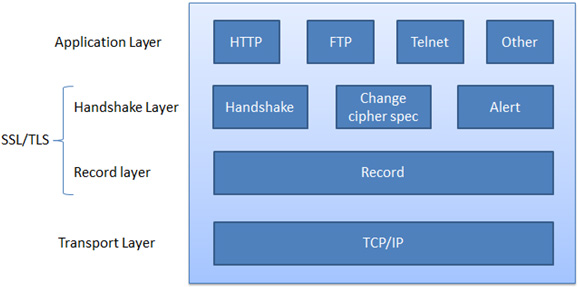
\includegraphics[scale=0.5]{img/ssl-tls-diag.jpg}
  \caption{SSL/TLS layer}
  \label{ssl-tls-diag}
\end{figure}  


\subsubsection{TLS Handshake protocol}

Ce protocole permet l'authentification et l'échange de clés nécessaires pour établir une session sécurisée. La figure \ref{handshake} décrit les différentes étapes de ce protocole:
\begin{figure}[H]
  \centering
  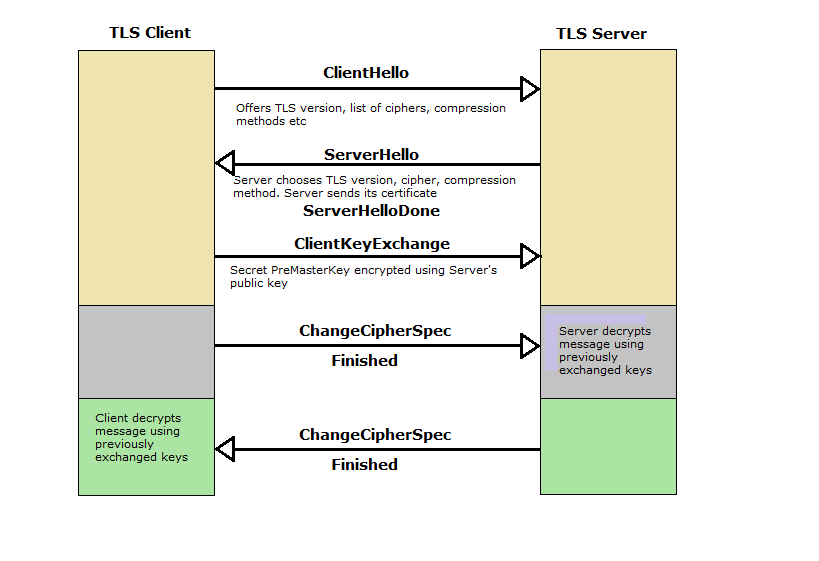
\includegraphics[scale=0.6]{img/tls-handshake.png}
  \caption{TLS handshake}
  \label{handshake}
\end{figure}  

Détails de chaque étape:
\begin{itemize}
\item le client envoie un message "ClientHello" au serveur, pour lui indiquer la dernière version TLS qu'il supporte, la liste des algorithmes de chiffrement qu'il supporte et les méthodes de compression qu'il supporte. Il envoie également un nombre aléatoire
\item le serveur renvoie un message "ServerHello", indiquant la version TLS, l'algorithme de chiffrement et la méthode de compression qui seront utilisés. Il envoie également son certificat (permettant l'authentification) et un nombre aléatoire
\item le serveur envoie un message "ServerHelloDone" pour indiquer qu'il a fini avec la première phase du handshake
\item le client génère un nombre appelé "PreMasterSecret", encrypté avec la clé publique du certificat du serveur
\item le client et le serveur génèrent alors leur secret partagé "Master Secret" à partir de leur nombre aléatoire et du "PreMasterSecret"
\item le client envoie un message "ChangeCipherSpec" indiquant que la suite de la communication sera cryptée, et envoie un message "Finished" qui est donc crypté
\item le serveur reçoit et décrypte le message et envoie son "ChangedCipherSpec"
\item le client reçoit et décrypte le message et c'est la fin du handshake
\end{itemize}
Les algorithmes utilisés pour l'échange de clés sont DH (Diffie-Hellman) et RSA. 

\subsubsection{TLS Record Protocol}

Ce protocole permet de sécuriser les données en utilisant les clés qu'on a crée pendant le handshake. Il permet également de vérifier l'intégrité des données. La figure \ref{record} présente son fonctionnement:
\begin{figure}[H]
\centering
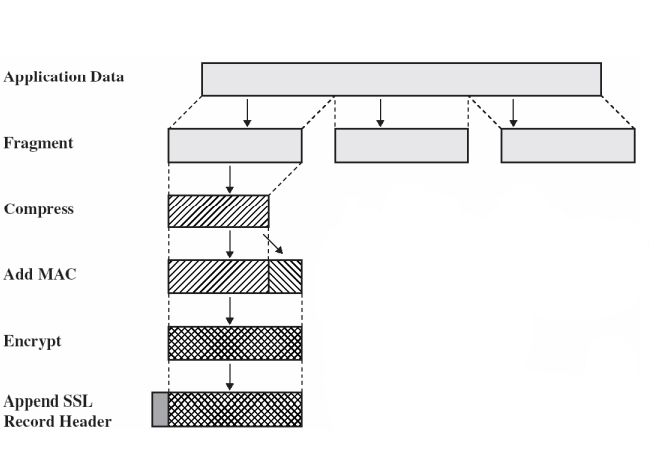
\includegraphics[scale=0.7]{img/tls-record.png}
\caption{TLS record}
\label{record}
\end{figure}

Détails de chaque étape:
\begin{itemize}
\item on divise le message à transmettre en fragments 
\item on compresse les fragments
\item on applique MAC (message authentification code) pour authentifier les messages 
\item on crypte les messages
\item on ajoute un en-t\^ete
\end{itemize}
Quand on reçoit un message, on fait l'opération inverse (décryptage, vérification d'authenfication avec le MAC, décompression, défragmentation). \\
Les algorithmes utilisés pour la phase de cryptage sont par exemple RC4, DES, 3DES, AES. \\
Le fonctionnement global décrit par les protocoles TLS handshake et TLS record est très similaire entre toutes les versions de SSL/TLS. \\

La sécurité du protocole est donc gérée par deux éléments:
\begin{itemize}
\item un chiffrement asymétrique qui permet, après authentification de la clé publique du serveur, la constitution d'un secret partagé entre le client et le serveur. C'est ce qui a lieu au cours du handshake
\item un chiffrement symétrique qui est utilisé dans la phase d'échange de données, car beaucoup moins coûteux et plus rapide. C'est ce qui a lieu dans la phase de cryptage du record. Les clés de chiffrement symétrique sont calculées à partir du secret partagé (de plus, une fonction de hachage est également utilisée pour assurer l'intégrité et l'authentification des données)
\end{itemize}

La faille Poodle exploite une faille de SSLv3 au niveau du mode de chiffrement symétrique CBC: le padding (complétion d'un bloc de bits pour respecter un format) permet de déchiffrer des messages. \\
La faille Freak exploite une faiblesse de SSLv3 au niveau du chiffrement asymétrique RSA: de nos jours on peut casser une clé RSA de 512 bits facilement, et SSLv3 utilise des clés RSA de 512 bits.

\subsection{La faille Poodle}

Comme on le voit sur la figure \ref{poodle}, le principe est que le client demande un service qui nécessite l'utilisation de SSL/TLS, et l'adversaire, en utilisant une attaque de type "man in the middle", force l'utilisation de SSLv3 et exploite ses failles.

\begin{figure}[H]
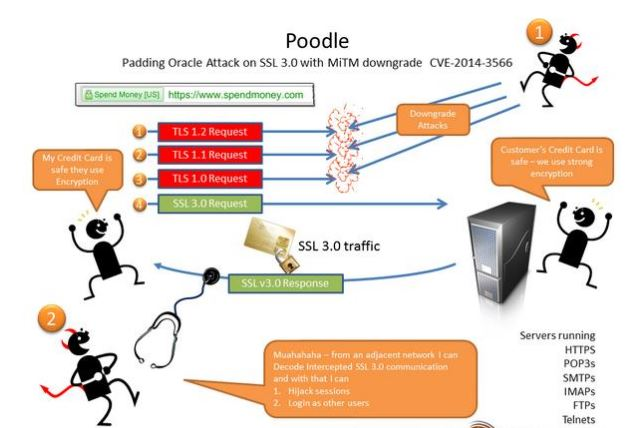
\includegraphics[scale=0.7]{img/poodle.jpg}
\caption{fonctionnement de la faille poodle}
\label{poodle}
\end{figure}

Avec cette méthode, l'adversaire n’a pas accès aux fichiers stockés dans l’appareil ciblé, mais il peut intercepter ses données de connexion, comme par exemple les cookies déposés dans le navigateur par un serveur lors d’une session. Sans posséder le mot de passe du client, l'adversaire peut effectuer des actions comme envoyer des messages sur Twitter en se faisant passer pour elle, lire et effacer son courrier électronique, etc.

\subsubsection{Détails de la vulnérabilité de SSLv3 exploitée}

Deux méthodes de chiffrement symétrique sont principalement utilisées dans SSLv3:
\begin{itemize}
\item la première est RC4 (Rivest Cipher 4) qui est un chiffrement par flot (stream cipher). Le principe d'un chiffrement par flot est de générer un flot de bits aléatoires $k$ et de réaliser un XOR entre ce flot et le message à chiffrer $m$. L'avantage est que chiffrement et déchiffrement sont très rapides: si $c = m \oplus k$, alors $m = c \oplus k$. Cependant, RC4 est actuellement considéré comme peu s\^ur et ne devrait plus \^etre utilisé
\item l'autre méthode est d'utiliser un algorithme comme DES ou AES avec un mode de chiffrement par blocs cha\^inés (CBC pour cipher block chaining), et c'est elle qui fait l'objet de l'attaque Poodle que l'on va détailler
\end{itemize}

\paragraph{Fonctionnement du chiffrement par blocs cha\^inés}

Les chiffrements et déchiffrements par blocs cha\^inés sont illustrés en figure \ref{cbc-enc} et \ref{cbc-dec} (Plaintext est le message en clair noté $m$ et Ciphertext est le message chiffré noté $c$) \\

\noindent On utilise la formule suivante pour chiffrer: \\
$c_i = Enc_K(m_i \oplus c_{i-1}),\ c_0 = IV$

\begin{figure}[H]
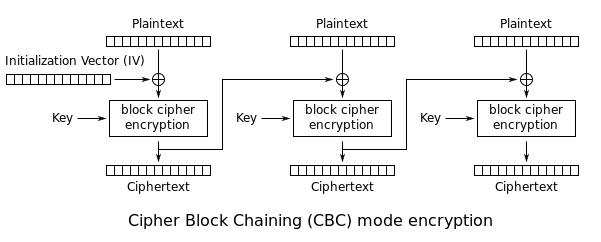
\includegraphics[scale=0.6]{img/cbc-enc.png}
\caption{CBC encryption}
\label{cbc-enc}
\end{figure}

\noindent On utilise la formule suivante pour déchiffrer: \\
$m_i = Dec_K(c_i) \oplus c_{i-1},\ c_0 = IV$ 

\begin{figure}[H]
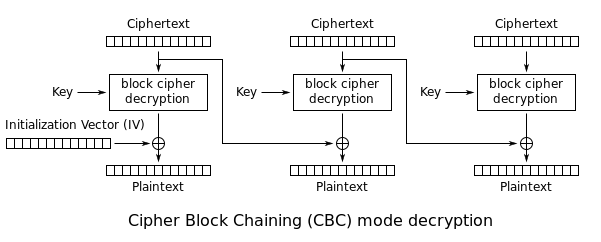
\includegraphics[scale=0.6]{img/cbc-dec.png}
\caption{CBC decryption}
\label{cbc-dec}
\end{figure}

Si un bit du message chiffré change, le bloc de message en clair correspondant est complètement corrompu et cela inverse le bit correspondant dans le bloc suivant de message en clair, mais le reste du bloc ne change pas. C'est ce qui est exploité par Poodle.

Supposons que l'adversaire ait trois blocs chiffrés $c_1$, $c_2$ et $c_3$ et qu'il souhaite décrypter le second bloc (et donc obtenir $m_2$). Il sait seulement que le dernier bloc est complété (padded) en utilisant la méthode PKCS7, c'est à dire que le dernier bloc est complété avec $n$ octets, chacun égal à $n$.
Le décryptage fonctionne comme ceci: $m_i = Dec(c_i) \oplus c_{i-1}$, avec $c_0 = IV$. Si l'adversaire change le dernier octet de $c_1$ et envoie ($IV$, $c_1$, $c_2$) au serveur, cela va affecter tout le bloc $m_1$ et le dernier octet de $m_2$. Ensuite le serveur va vérifier le dernier bloc décrypté ($m_2$) et retourner oui ou non si la complétion ("padding") est correcte.
Si $b_{-1}$ est le dernier octet de $c_1$, l'adversaire le change comme suit: $b_{-1} = b_{-1} \oplus z_{-1} \oplus$ 0x01, où $z_{-1}$ est la valeur du dernier octet de $m_2$. Si $z_{-1}$ est correct, le serveur ne va pas trouver d'erreur de padding (parce que le dernier octet de $m_2$ sera égal à 0x01, ce qui est un padding correct). Dans l'autre cas, le serveur va trouver une erreur de padding et l'adversaire va essayer une autre valeur de $z_{-1}$. Dans le pire des cas, il doit faire 255 essais pour trouver la bonne valeur de $z_{-1}$.

Une fois qu'il connait le dernier octet de $m_2$, l'adversaire peut obtenir l'avant dernier octet de $m_2$. Il change les deux derniers octets de $c_1$: $b_{-1} = b_{-1} \oplus z_{-1} \oplus$ 0x02 et $b_{-2} = b_{-2} \oplus z_{-2} \oplus$ 0x02. Après 255 essais au maximum il trouve $z_{-2}$ et ainsi de suite. 

Si chaque bloc fait 128 bits (AES), soit 16 octets, l'adversaire va obtenir $m_2$ en moins de 255x16 = 4080 essais. Cette attaque ne co\^ute presque rien et peut \^etre réalisée en quelques secondes.

La publication de Google qui a officialisé le faille offre les détails nécessaires pour récupérer les cookies d'une cible: This POODLE Bites: Exploiting The SSL 3.0 Fallback, Security Advisory, Bodo Möller, Thai Duong, Krzysztof Kotowicz, Google, September 2014.


\subsection{La faille Freak}

Le principe global de fonctionnement est le m\^eme que pour la faille poodle (une attaque de type "man in the middle" force l'utilisation de SSLv3). La seule différence est que ce n'est pas la m\^eme vulnérabilité de SSLv3 qui est exploitée.

\subsubsection{Détails de la vulnérabilité de SSLv3 exploitée}

Ici, il s'agit du fait que si l'algorithme de chiffrement asymétrique utilisé pendant le handshake est RSA, alors sous SSLv3, la clé est de 512 bits. Cette taille de 512 bits a été choisie par la NSA dans les années 1990, et était juste suffisante pour que eux seuls puissent casser ces clés. Seulement, de nos jours, casser une clé RSA de 512 bits est très abordable. Dans les versions ultérieures de SSLv3 (TLS 1.0, 1.1 et 1.2), ces clés sont plus grandes (1024/2048 bits), d'où l'inter\^et pour l'adversaire de forcer l'utilisation de SSLv3 par une attaque "man in the middle".

\paragraph{Fonctionnement du chiffrement RSA}

Le chiffrement RSA sert à établir un secret entre deux entités, par convention Alice (A) et Bob (B). Dans le cas du protocole SSL/TLS, on utilise le chiffrement RSA pour étalbir la clé qui sert au chiffrement symétrique (CBC, AES, DES) des communications. \\ 
RSA est un chiffrement asymétrique, c'est à dire qu'il utilise deux clés: une publique pour chiffrer et une privée pour déchiffrer. Le principe étant que déchiffrer avec comme seule connaissance la clé publique soit calculatoirement impossible. \\

Le chiffrement RSA fonctionne en 3 étapes:
\begin{itemize}
\item \textbf{création des clés} \\
La création des clés se fait du c\^oté d'Alice par l'algorithme suivant:
\begin{itemize}
\item choisir $p$ et $q$, deux nombres premiers distincts
\item calculer le produit $n = pq$, appelé module de chiffrement 
\item calculer $\phi(n) = (p - 1)(q -1)$ (c'est la valeur de l'indicatrice d'Euler en $n$) 
\item choisir un entier naturel $e$ premier avec $\phi(n)$ et strictement inférieur à  $\phi(n)$, appelé exposant de chiffrement
\item calculer l'entier naturel $d$, inverse de $e$ modulo  $\phi(n)$, et strictement inférieur à  $\phi(n)$, appelé exposant de déchiffrement ($d$ peut se calculer efficacement par l'algorithme d'Euclide étendu)
\end{itemize}
Comme $e$ est premier avec  $\phi(n)$, d'après le théorème de Bachet-Bézout il existe deux entiers $d$ et $k$ tels que $ed + k \phi(n) = 1$, c'est-à-dire que $ed = 1\ mod\ \phi(n)$ : $e$ est bien inversible modulo $\phi(n)$.

Le couple ($n$,$e$) est la clé publique du chiffrement, alors que le couple ($n$,$d$) est sa clé privée.

\item \textbf{chiffrement du message} \\
Si $M$ est un entier naturel strictement inférieur à $n$ représentant un message, alors le message chiffré sera représenté par: \\
$C = M^e\ mod\ n$ \\
L'entier naturel $C$ étant choisi strictement inférieur à $n$.

\item \textbf{déchiffrement du message} \\
Pour déchiffrer $C$, on utilise $d$, l'inverse de $e\ mod\ (p-1)(q-1)$, et on retrouve le message clair $M$ par: \\
$M = C^d\ mod\ n$ \\


Pour chiffrer un message, il suffit de connaître $e$ et $n$ alors que pour déchiffrer, il faut $d$ et $n$. \\
Pour calculer $d$ à l'aide de $e$ et $n$, il faut trouver l'inverse modulaire de $e$ modulo $(p - 1)(q - 1)$ ce que l'on ne sait pas faire sans connaître les entiers $p$ et $q$, c'est-à-dire la décomposition de $n$ en facteurs premiers. \\
Une attaque par force brute consisterait donc à retrouver $p$ et $q$ en ne connaissant que $n$. Dans le pire des cas, sur une clé de 512 bits, on peut tester tous les nombres premiers inférieurs à $\sqrt{2^{512}}$\\
%La sécurité de l'algorithme RSA contre les attaques par la force brute repose donc sur le fait que casser RSA de cette manière nécessite la factorisation du nombre $n$ en le produit initial des nombres $p$ et $q$, et qu'avec les algorithmes classiques, le temps que prend cette factorisation croît exponentiellement avec la longueur de la clé. \\


\end{itemize}


\section{Que faire face aux failles Poodle et Freak ?}

google article Poodle:

The attack described above requires an SSL 3.0 connection to be established, so sisabling the SSL 3.0 protocol in the client or in the server (or both) will completely avoid it. If either side supports only SSL 3.O, then all hope is gone, and a serious updade required to avoid insecure encryption. If SSL 3.O is neither disable nor the only possible protocol version, then the attack is possible if the client uses a downgrade dance for interoperability. 

Disabling SSL 3.O entirely right away may not be practical if it is needed occasinaly to work with legacy systems. Also, similar protocol version downgrades are still a concernwith newer protocol versions (although not nearly as severe as with SSL 3.0). The TLS\_FALLBACK\_SCSV mechanism from [draft-ietf-tls-downgrade-scsv-00] addresses the broader issue across protocol versions, and we consider it crucial especially for systems that maintain SSL 3.O compatibility. The folloainw recommendations summaeize how TLS\_FALLBACK\_SCSV works.

TLS clients that use a downgrade dance to improve interoperability should include the value 0x56, 0x00 (TLS\_FALLBACK\_SCSV) in CLientHello.cipher\_suites in any fallback handshake. THis value serves as a signal allowing updated servers to reject the connection in case of a downgrade attack. Clients should always fall back to the next lower version (if starting at TLS 1.2, try 1.1 next then 1.0 then SSL 3.0) because skipping a protocol version forgoes its better security. (with TLS\_FALLBACK\_SCSV, skipping a version also could entirely prevent a succesful handshake if it happens to be the version that should be use with the server in question)

In TLS servers,whenever an incoming connection includes 0x56,0x00(TLS\_FALLBACK\_SCSV)in ClientHello.cipher\_suites,compareClientHello.client\_version to the highest protocol version supported by the server.If the server supports a version higher than the one indicated by the client,reject the connection with a fatal alert (preferably,inappropriate\_fallback(86) from [draftietftlsdowngradescsv00]

This use of TLS\_FALLBACK\_SCSV will ensure that SSL3.0 is used only when a legacy implementation is involved:attackers can no longer force a protocol downgrade.(Attacksremain possible if both parties allow SSL3.0 but one of them is not updated to support TLS\_FALLBACK\_SCSV, provided that the client implements a downgrade dance down to SSL 3.0.




freak websites 

What should I do?

If you run a server …

You should immediately disable support for TLS export cipher suites. While you’re at it, you should also disable other cipher suites that are known to be insecure and enable forward secrecy. For instructions on how to secure popular HTTPS server software, we recommend Mozilla’s security configuration guide and their SSL configuration generator. We also recommend testing your configuration with the Qualys SSL Labs SSL Server Test tool.
If you use a browser …

Make sure you have the most recent version of your browser installed, and check for updates frequently. Updates that fix the FREAK attack should be available for all major browsers soon.
If you’re a sysadmin or developer …

Make sure any TLS libraries you use are up to date. Unpatched OpenSSL, Microsoft Schannel, and Apple SecureTransport all suffer from the vulnerability. Note that these libraries are used internally by many other programs, such as wget and curl. You also need to ensure that your software does not offer export cipher suites, even as a last resort, since they can be exploited even if the TLS library is patched. We have provided tools for software developers that may be helpful for testing.


\input{bilan}



\end{document}
